\chapter{Planos de organização e tecidos animais}\label{ch:b1:body-plans-tissues}

Quatro animais sobre a bancada do laboratório: uma hidra de um
centímetro, uma minhoca, um lagostim, uma rã. Sob as diferenças de
tamanho e de hábito, eles são construídos a partir de um punhado de
decisões comuns --- se o corpo tem frente e trás, de quantas camadas de
células ele se formou, se há uma cavidade em torno do tubo digestório,
se o corpo é feito de segmentos repetidos, onde fica o esqueleto --- e
cada um deles é construído com os mesmos quatro tipos de \omterm{def:b1:body-plans-tissues:tissue}{tecido}. Este
capítulo expõe os \omterm{def:b1:mammal-organization:bodyplan}{planos de organização} dos animais e os \omterm{def:b1:body-plans-tissues:tissue}{tecidos} que os
constroem, e termina onde os capítulos anteriores pararam: na \omterm{prop:b1:body-plans-tissues:gutwall}{parede do
tubo digestório} de um mamífero, vista como \omterm{def:b1:body-plans-tissues:tissue}{tecidos} montados em um \omterm{def:b1:mammal-organization:organ}{órgão}.

\section{Planos de organização}

\begin{definition}[Simetria e cefalização]\label{def:b1:body-plans-tissues:symmetry}
Um animal tem \emph{simetria radial}\index{simetria radial} quando o
corpo dele é organizado em torno de um eixo central, sem esquerda e
direita, como uma hidra ou uma água-viva: ele encontra o ambiente
igualmente por todos os lados, e em geral é fixo ou deriva na água. Ele
tem \emph{simetria bilateral}\index{simetria bilateral} quando um plano
o divide em duas metades espelhadas, definindo uma frente (anterior) e
uma traseira (posterior), um dorso (dorsal) e um ventre (ventral): o
plano de um animal que se desloca com a cabeça à frente, com os \omterm{def:b1:mammal-organization:organ}{órgãos}
dos sentidos e os centros nervosos concentrados na frente (\omterm{def:b1:mammal-organization:bodyplan}{cefalização}).
\end{definition}

\begin{definition}[Folhetos embrionários, cavidades corporais]\label{def:b1:body-plans-tissues:layers}
O embrião de um animal forma duas ou três camadas de células, os
\emph{folhetos embrionários}\index{folheto embrionário}, dos quais
derivam todos os \omterm{def:b1:body-plans-tissues:tissue}{tecidos}: o \emph{ectoderma}\index{ectoderma} externo
(pele, sistema nervoso), o \emph{endoderma}\index{endoderma} interno
(revestimento do tubo digestório e das expansões dele) e, em todos
exceto as esponjas e os cnidários, um \emph{mesoderma}\index{mesoderma}
intermediário (músculo, esqueleto, \omterm{def:b1:body-plans-tissues:connective}{tecido conjuntivo}, sangue, rins,
gônadas). Os cnidários são \emph{diblásticos}; os demais,
\emph{triblásticos}. Entre os animais triblásticos, o mesoderma pode
preencher o espaço entre o tubo digestório e a parede do corpo
(\emph{acelomados}: platelmintos), ou deixar uma cavidade entre eles: um
\emph{celoma}\index{celoma} quando a cavidade é inteiramente revestida
por mesoderma (anelídeos, moluscos, artrópodes, equinodermos,
vertebrados). O celoma suspende o tubo digestório em um compartimento
próprio, permite que ele se mova independentemente da parede do corpo, e
dá aos animais de corpo mole um \omterm{def:b1:body-plans-tissues:segments}{esqueleto hidrostático}.
\end{definition}

\begin{omfigure}
\begin{tikzpicture}[font=\footnotesize, line cap=round]
  \node[font=\small, anchor=south] at (1.4,2.75) {acelomado (platelminto)};
  \node[font=\small, anchor=south] at (6.6,2.75) {celomado (anelídeo, vertebrado)};
  % acoelomate: body wall ectoderm, solid mesoderm, gut endoderm
  \draw[thick, fill=omDef!25] (1.4,1.3) ellipse (1.35 and 1.25);
  \fill[omProp!35] (1.4,1.3) ellipse (1.15 and 1.05);
  \draw[thick, fill=omExo!30] (1.4,1.3) ellipse (0.4 and 0.35);
  \node at (1.4,1.3) {tubo digestório};
  \node at (1.4,0.62) {mesoderma};
  % coelomate: body wall, coelom, gut with mesoderm layer
  \draw[thick, fill=omDef!25] (6.6,1.3) ellipse (1.35 and 1.25);
  \fill[omProp!35] (6.6,1.3) ellipse (1.15 and 1.05);
  \fill[white] (6.6,1.3) ellipse (0.95 and 0.85);
  \draw[thick, fill=omProp!35] (6.6,1.3) ellipse (0.55 and 0.5);
  \draw[thick, fill=omExo!30] (6.6,1.3) ellipse (0.4 and 0.35);
  \node at (6.6,1.3) {tubo digestório};
  \node at (6.6,0.62) {celoma};
  % legend
  \fill[omDef!25] (8.9,2.2) rectangle +(0.35,0.25); \node[anchor=west] at (9.3,2.32) {ectoderma};
  \fill[omProp!35] (8.9,1.7) rectangle +(0.35,0.25); \node[anchor=west] at (9.3,1.82) {mesoderma};
  \fill[omExo!30] (8.9,1.2) rectangle +(0.35,0.25); \node[anchor=west] at (9.3,1.32) {endoderma};
  \draw (8.9,0.7) rectangle +(0.35,0.25); \node[anchor=west] at (9.3,0.82) {celoma (cavidade)};
\end{tikzpicture}

{\small Cortes transversais de dois \omterm{def:b1:mammal-organization:bodyplan}{planos de organização} triblásticos.
No acelomado o \omterm{def:b1:body-plans-tissues:layers}{mesoderma} preenche o espaço entre a parede do corpo e o
tubo digestório; no celomado uma cavidade revestida de \omterm{def:b1:body-plans-tissues:layers}{mesoderma} os
separa, de modo que o tubo fica suspenso e o líquido da cavidade pode
funcionar como esqueleto.}
\end{omfigure}

\begin{definition}[Protostômios e deuterostômios]\label{def:b1:body-plans-tissues:proto}
Entre os animais celomados, o destino da primeira abertura do tubo
digestório embrionário separa duas grandes linhagens: nos
\emph{protostômios}\index{protostômio} (anelídeos, moluscos,
artrópodes) ela se torna a boca, o \omterm{def:b1:body-plans-tissues:layers}{celoma} se forma pela clivagem do
\omterm{def:b1:body-plans-tissues:layers}{mesoderma}, e as primeiras divisões do ovo são espiraladas e têm destino
fixado cedo; nos \emph{deuterostômios}\index{deuterostômio}
(equinodermos, vertebrados) ela se torna o ânus, o \omterm{def:b1:body-plans-tissues:layers}{celoma} se forma por
evaginação do tubo digestório, e as primeiras células mantêm o destino
flexível.
\end{definition}

\begin{definition}[Segmentação, esqueletos]\label{def:b1:body-plans-tissues:segments}
Um corpo é \emph{segmentado}\index{segmentação} quando é construído a
partir de unidades repetidas ao longo do eixo dele (os anéis de uma
minhoca, os segmentos de um lagostim, as vértebras e os blocos
musculares de um peixe), cada uma com o próprio conjunto de músculos,
nervos e, muitas vezes, apêndices. Os segmentos podem ser iguais ou
especializados em regiões (cabeça, tórax, abdome). O
\emph{esqueleto}\index{esqueleto}, contra o qual os músculos tracionam,
é \emph{hidrostático}\index{esqueleto hidrostático} (um líquido sob
pressão em um \omterm{def:b1:body-plans-tissues:layers}{celoma}, como na minhoca), um
\emph{exoesqueleto}\index{exoesqueleto} (uma \omterm{def:b1:flowering-plant-organization:tissues}{cutícula} rígida por fora do
corpo, articulada, trocada para crescer, como nos artrópodes) ou um
\emph{endoesqueleto}\index{endoesqueleto} (cartilagem ou osso dentro do
corpo, que cresce junto com ele, como nos vertebrados).
\end{definition}

\begin{omfigure}
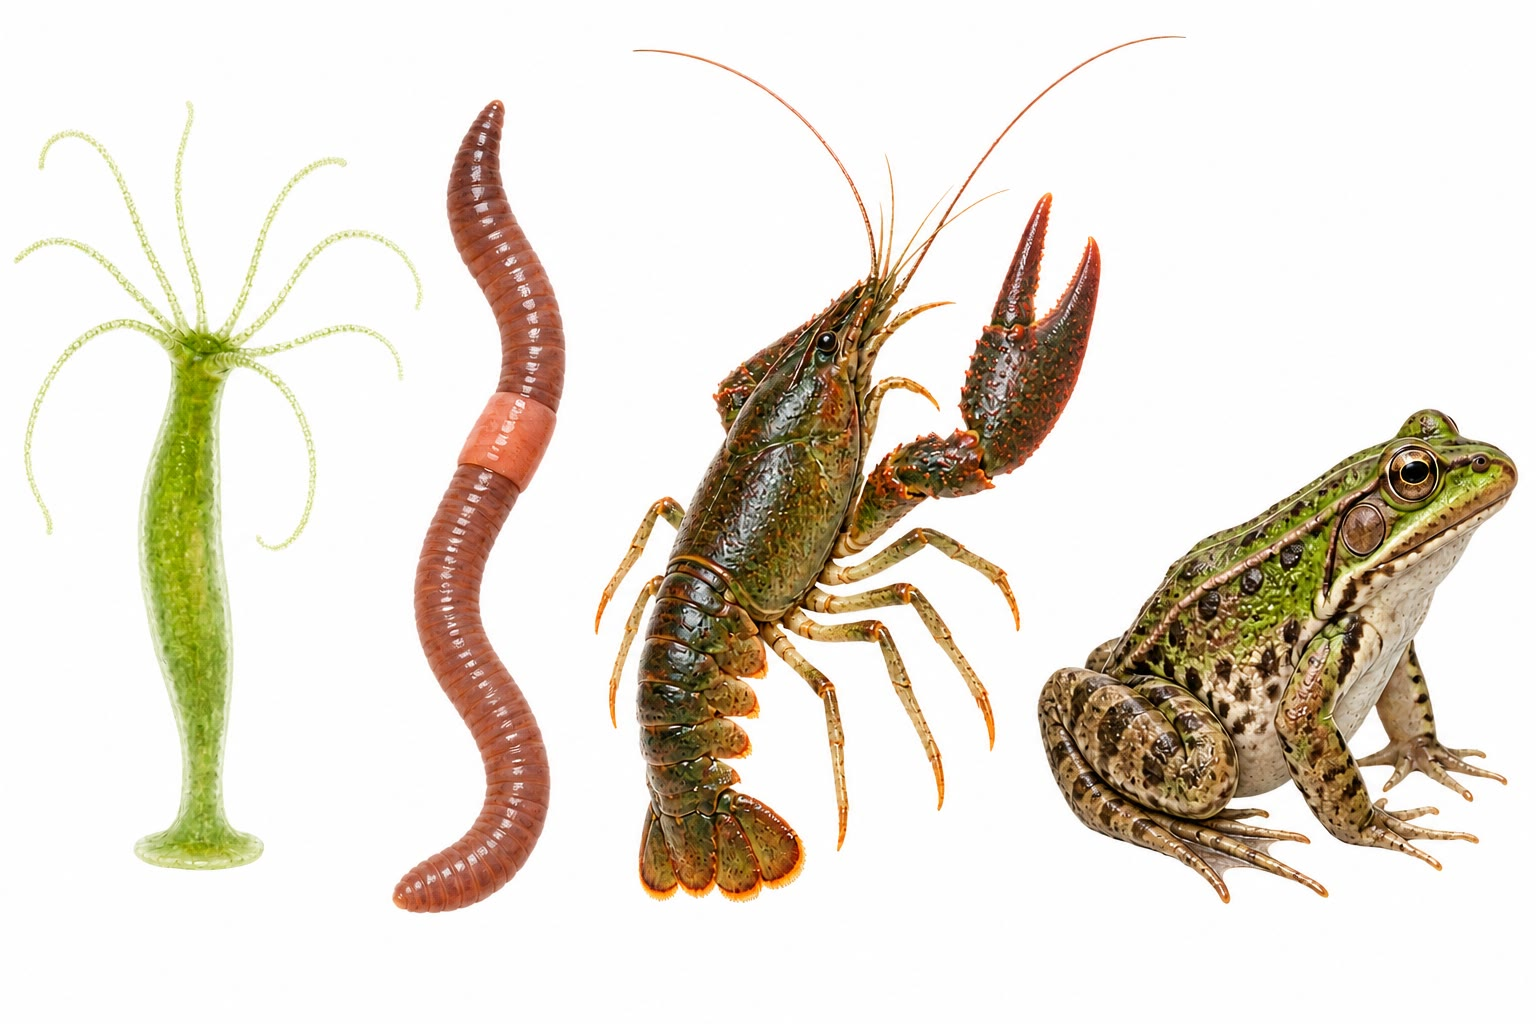
\includegraphics[width=0.78\linewidth]{images/book3/ai/b3-04-body-plans.jpg}

{\small Quatro \omterm{def:b1:mammal-organization:bodyplan}{planos de organização}. Uma hidra (radial, duas camadas,
sem \omterm{def:b1:body-plans-tissues:layers}{celoma}), uma minhoca (bilateral, celomada, segmentada, \omterm{def:b1:body-plans-tissues:segments}{esqueleto
hidrostático}), um lagostim (\omterm{def:b1:body-plans-tissues:segments}{segmentado} com regiões especializadas,
\omterm{def:b1:body-plans-tissues:segments}{exoesqueleto} articulado) e uma rã (\omterm{def:b1:body-plans-tissues:proto}{deuterostômio}, \omterm{def:b1:body-plans-tissues:segments}{endoesqueleto} ósseo).}
\end{omfigure}

\begin{proposition}[Quatro planos comparados]\label{prop:b1:body-plans-tissues:four}
\begin{center}
\footnotesize
\begin{tabular}{lllll}
\hline
 & hidra & minhoca & lagostim & rã \\
\hline
simetria & radial & bilateral & bilateral & bilateral \\
\omterm{def:b1:body-plans-tissues:layers}{folhetos embrionários} & 2 & 3 & 3 & 3 \\
\omterm{def:b1:body-plans-tissues:layers}{celoma} & nenhum & sim & reduzido & sim \\
linhagem & --- & \omterm{def:b1:body-plans-tissues:proto}{protostômio} & \omterm{def:b1:body-plans-tissues:proto}{protostômio} & \omterm{def:b1:body-plans-tissues:proto}{deuterostômio} \\
segmentos & não & iguais & especializados & vértebras, blocos musculares \\
esqueleto & hidrostático & hidrostático & \omterm{def:b1:body-plans-tissues:segments}{exoesqueleto} & \omterm{def:b1:body-plans-tissues:segments}{endoesqueleto} \\
tubo digestório & uma abertura & boca a ânus & boca a ânus & boca a ânus \\
circulação & nenhuma & fechada & aberta & fechada, com coração \\
sistema nervoso & rede & cordão ventral & cordão ventral & cordão dorsal \\
\hline
\end{tabular}
\end{center}
Os planos não são degraus de uma escada: cada um é uma maneira completa
e bem-sucedida de ser um animal, e o lagostim e a rã são contemporâneos
um do outro, não ancestrais.
\end{proposition}

\begin{example}[Ler um animal a partir do plano dele]\label{ex:b1:body-plans-tissues:reading}
Um animal com uma extremidade cefálica, um tubo digestório completo, um
corpo de anéis semelhantes e nenhuma parte dura: um \omterm{def:b1:body-plans-tissues:proto}{protostômio} celomado
que se move por um \omterm{def:b1:body-plans-tissues:segments}{esqueleto hidrostático}, com o líquido celômico de
cada segmento pressurizado alternadamente por músculos circulares e
longitudinais --- uma minhoca escavando. Um animal com uma \omterm{def:b1:flowering-plant-organization:tissues}{cutícula}
articulada e segmentos especializados: um artrópode, cujo crescimento
precisa passar por mudas. Bilateral, com blocos musculares \omterm{def:b1:body-plans-tissues:segments}{segmentados}
em torno de um eixo dorsal de vértebras: um vertebrado, cujo
\omterm{def:b1:body-plans-tissues:segments}{endoesqueleto} cresce continuamente.
\end{example}

\section{Os quatro tipos de tecido}

\begin{definition}[Tecido]\label{def:b1:body-plans-tissues:tissue}
Um \emph{tecido}\index{tecido} é um conjunto de células de estrutura e
origem semelhantes, junto com o material extracelular que elas produzem,
organizado para desempenhar uma função comum. Os tecidos animais se
dividem em quatro tipos: epitelial, conjuntivo, muscular e nervoso. Todo
\omterm{def:b1:mammal-organization:organ}{órgão} é uma combinação de pelo menos dois deles.
\end{definition}

\begin{definition}[Tecido epitelial]\label{def:b1:body-plans-tissues:epithelium}
Um \emph{epitélio}\index{epitélio} é uma lâmina de células muito
justapostas que recobre uma superfície ou reveste uma cavidade,
apoiada sobre uma camada fina de \omterm{def:b1:body-plans-tissues:connective}{matriz extracelular}, a
\emph{lâmina basal}\index{lâmina basal}. As células dele são
\emph{polarizadas}\index{polaridade celular}: a face apical olha para o
exterior ou para o lúmen, a face basal para a lâmina, e as duas carregam
proteínas diferentes. Elas são unidas por
\emph{junções celulares}\index{junção celular}: as
\emph{junções oclusivas} perto do ápice, que vedam o espaço entre as
células de modo que nada atravesse a lâmina a não ser através delas; as
\emph{junções aderentes} e os \emph{desmossomos}, que prendem as células
mecanicamente; as \emph{junções comunicantes}, canais que deixam íons e
moléculas pequenas passarem de célula a célula. Os epitélios são
classificados pelo número de camadas (simples, estratificado) e pela
forma das células (pavimentosas, cúbicas, prismáticas), e incluem as
glândulas, que são células epiteliais especializadas em secreção. Eles
recobrem, protegem, absorvem e secretam.
\end{definition}

\begin{omfigure}
\begin{tikzpicture}[font=\footnotesize, line cap=round]
  % three columnar cells
  \foreach \x in {0,1.6,3.2} {
    \draw[thick, fill=omDef!10] (\x,0) rectangle (\x+1.5,3.2);
    \fill[omDef!60] (\x+0.75,0.9) ellipse (0.32 and 0.42);
    % microvilli
    \foreach \m in {0.15,0.35,0.55,0.75,0.95,1.15,1.35} \draw[omDef!70!black, thick] (\x+\m,3.2) -- (\x+\m,3.5);
  }
  % junctions between cell 1-2 and 2-3
  \foreach \x in {1.55,3.15} {
    \draw[very thick, omThm] (\x-0.05,2.9) -- (\x+0.1,2.9);
    \draw[very thick, omProp] (\x-0.05,2.5) -- (\x+0.1,2.5);
    \draw[very thick, omProp] (\x-0.05,1.9) -- (\x+0.1,1.9);
    \draw[very thick, omExo] (\x-0.05,1.2) -- (\x+0.1,1.2);
  }
  % basal lamina
  \draw[very thick, gray!70] (-0.2,-0.05) -- (4.9,-0.05);
  \fill[pattern=north east lines, pattern color=gray!50] (-0.2,-0.6) rectangle (4.9,-0.1);
  % labels
  \node[anchor=south] at (2.4,3.55) {face apical: microvilosidades, voltada para o lúmen};
  \node[anchor=west, omThm] at (5.1,2.9) {junção oclusiva: veda a fresta};
  \node[anchor=west, omProp] at (5.1,2.5) {junção aderente: cinturão de actina};
  \node[anchor=west, omProp] at (5.1,1.9) {desmossomo: rebite mecânico};
  \node[anchor=west, omExo] at (5.1,1.2) {junção comunicante: canal entre células};
  \node[anchor=west, gray!80!black] at (5.1,-0.05) {lâmina basal};
  \node[anchor=west, gray!80!black] at (5.1,-0.45) {tecido conjuntivo abaixo};
  \node[anchor=east] at (-0.3,0.9) {núcleo};
\end{tikzpicture}

{\small Um \omterm{def:b1:body-plans-tissues:epithelium}{epitélio} prismático simples, como o do intestino. Cada célula
tem uma face apical com microvilosidades e uma face basal sobre a \omterm{def:b1:body-plans-tissues:epithelium}{lâmina
basal}; as vizinhas são vedadas por junções oclusivas, presas por junções
aderentes e desmossomos, e conectadas por junções comunicantes.}
\end{omfigure}

\begin{definition}[Tecido conjuntivo]\label{def:b1:body-plans-tissues:connective}
O \emph{tecido conjuntivo}\index{tecido conjuntivo} é feito de células
esparsas numa \emph{matriz extracelular}\index{matriz extracelular}
abundante que elas mesmas secretam: fibras proteicas ---
\emph{colágeno}\index{colágeno} (resistência à tração; um quarto de toda
a proteína de um mamífero), \emph{elastina}\index{elastina} (retorno
elástico) --- embebidas numa \emph{substância fundamental} hidratada de
polissacarídeos. As proporções definem os tipos dele: o \omterm{def:b1:body-plans-tissues:tissue}{tecido}
conjuntivo frouxo sob os \omterm{def:b1:body-plans-tissues:epithelium}{epitélios} e em volta dos \omterm{def:b1:mammal-organization:organ}{órgãos} (fibroblastos,
poucas fibras, muita substância fundamental); o \omterm{def:b1:body-plans-tissues:tissue}{tecido} conjuntivo denso
dos tendões e dos ligamentos (colágeno paralelo); o \omterm{def:b1:body-plans-tissues:tissue}{tecido} adiposo
(células que armazenam gordura); a cartilagem (um gel firme de colágeno
e polissacarídeos, sem vasos); o osso (colágeno mineralizado com fosfato
de cálcio, células vivas em lacunas, vasos); e o sangue, cuja matriz é o
plasma. Ele une, sustenta, armazena, transporta e defende.
\end{definition}

\begin{definition}[Tecido muscular]\label{def:b1:body-plans-tissues:muscle}
O \emph{tecido muscular}\index{tecido muscular} é feito de células
alongadas repletas de filamentos proteicos contráteis (actina e
miosina). São três tipos: o \emph{músculo esquelético}, de fibras longas
e multinucleadas com estriações transversais, preso ao esqueleto e sob
controle voluntário; o \emph{músculo cardíaco}, de células estriadas e
ramificadas unidas topo a topo por junções que passam o batimento de
célula a célula, contraindo-se em ritmo próprio; e o
\emph{músculo liso}, de células fusiformes e não estriadas nas paredes
dos \omterm{def:b1:mammal-organization:organ}{órgãos} ocos (intestino, vasos, útero), contraindo-se lentamente e
de modo involuntário. O mecanismo da contração é tratado no volume do
Ano 2.
\end{definition}

\begin{definition}[Tecido nervoso]\label{def:b1:body-plans-tissues:nervous}
O \emph{tecido nervoso}\index{tecido nervoso} é feito de
\emph{neurônios}\index{neurônio}, células com um corpo e prolongamentos
longos (os dendritos, que recebem sinais, e um axônio, que os leva
adiante) que conduzem sinais elétricos e os transmitem a outras células
nas sinapses, e de \emph{células gliais}\index{célula glial}, várias
vezes mais numerosas, que sustentam, isolam e alimentam os neurônios.
Ele percebe, integra e comanda.
\end{definition}

\begin{omfigure}
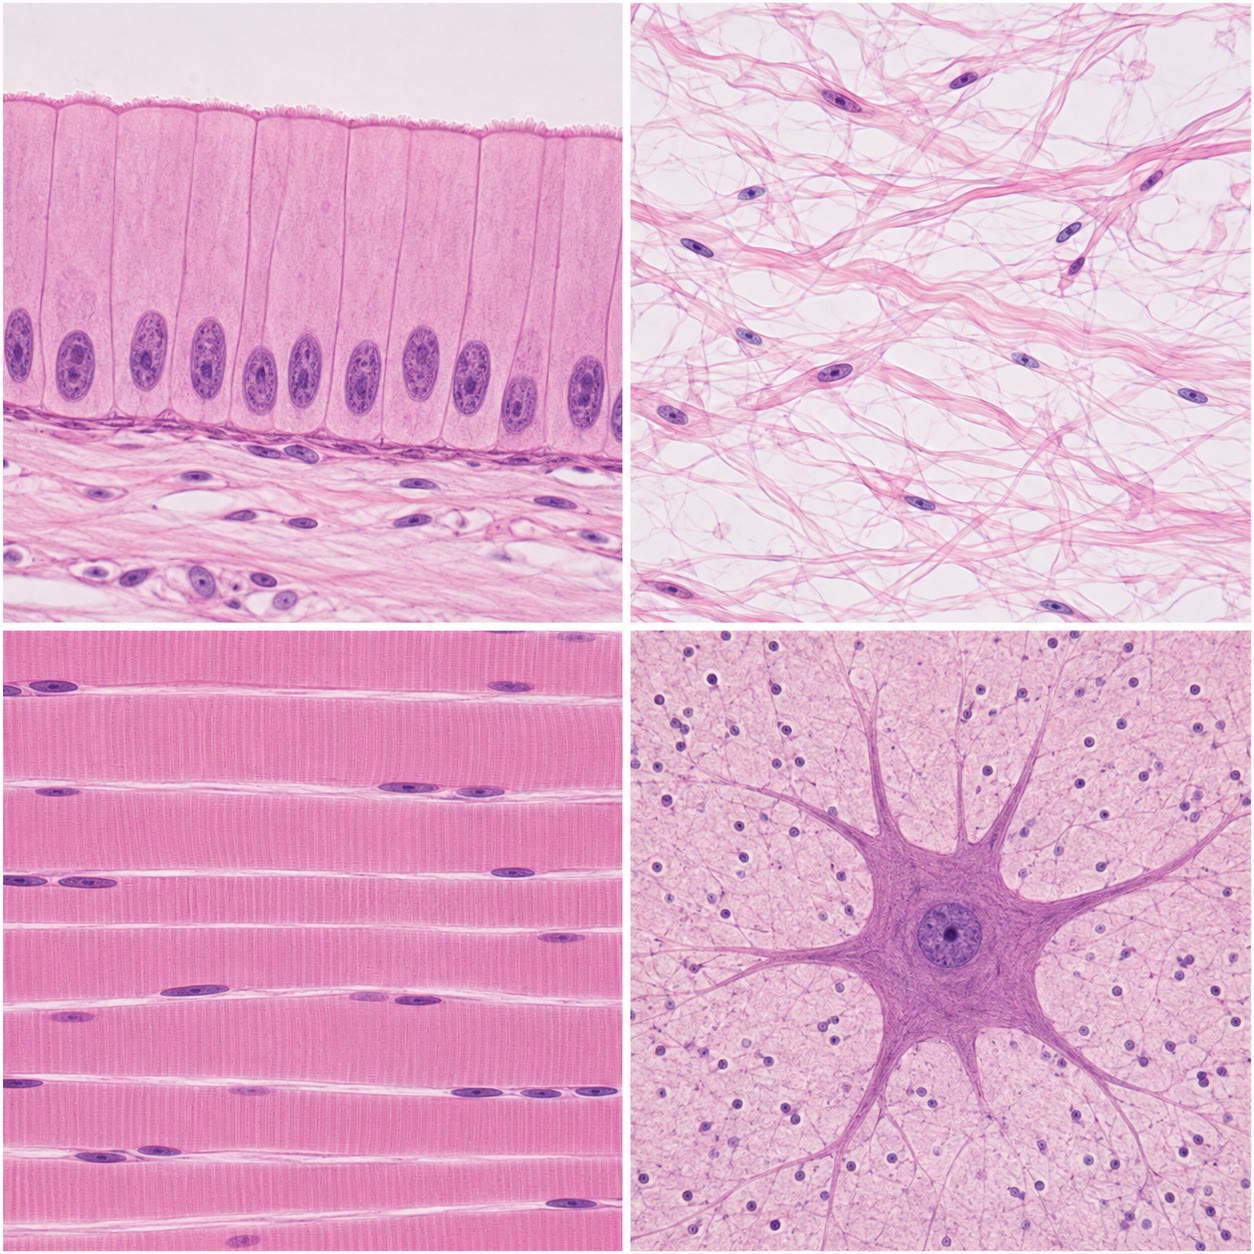
\includegraphics[width=0.6\linewidth]{images/book3/ai/b3-04-tissues.jpg}

{\small Os quatro tipos de \omterm{def:b1:body-plans-tissues:tissue}{tecido} ao microscópio. Em cima, à esquerda:
\omterm{def:b1:body-plans-tissues:epithelium}{epitélio} prismático simples, uma única fileira de células altas. Em
cima, à direita: \omterm{def:b1:body-plans-tissues:connective}{tecido conjuntivo} frouxo, células esparsas entre fibras
onduladas de \omterm{def:b1:body-plans-tissues:connective}{colágeno}. Embaixo, à esquerda: fibras musculares
esqueléticas, estriadas, com os núcleos nas bordas. Embaixo, à direita:
um \omterm{def:b1:body-plans-tissues:nervous}{neurônio} entre \omterm{def:b1:body-plans-tissues:nervous}{células gliais}.}
\end{omfigure}

\begin{example}[De onde vêm os tecidos]\label{ex:b1:body-plans-tissues:origin}
Os \omterm{def:b1:body-plans-tissues:epithelium}{epitélios} derivam dos três \omterm{def:b1:body-plans-tissues:layers}{folhetos embrionários} (a pele do
\omterm{def:b1:body-plans-tissues:layers}{ectoderma}, o revestimento do tubo digestório do \omterm{def:b1:body-plans-tissues:layers}{endoderma}, o
revestimento dos vasos e do \omterm{def:b1:body-plans-tissues:layers}{celoma} do \omterm{def:b1:body-plans-tissues:layers}{mesoderma}); o \omterm{def:b1:body-plans-tissues:connective}{tecido conjuntivo}, o
muscular e o sangue vêm do \omterm{def:b1:body-plans-tissues:layers}{mesoderma}; o \omterm{def:b1:body-plans-tissues:nervous}{tecido nervoso}, do \omterm{def:b1:body-plans-tissues:layers}{ectoderma}. A
pele da rã é um \omterm{def:b1:body-plans-tissues:epithelium}{epitélio} ectodérmico sobre \omterm{def:b1:body-plans-tissues:connective}{tecido conjuntivo}
mesodérmico; o tubo digestório dela, um \omterm{def:b1:body-plans-tissues:epithelium}{epitélio} endodérmico envolvido
em músculo mesodérmico; o encéfalo dela, \omterm{def:b1:body-plans-tissues:layers}{ectoderma} dobrado para dentro.
\end{example}

\section{Dos tecidos a um órgão: a parede do tubo digestório}

\begin{proposition}[As quatro camadas da parede do tubo digestório]\label{prop:b1:body-plans-tissues:gutwall}
\index{parede do tubo digestório}
Do lúmen para fora, a \omterm{prop:b1:body-plans-tissues:gutwall}{parede do tubo digestório} dos vertebrados é
construída com quatro camadas concêntricas, cada uma uma combinação de
\omterm{def:b1:body-plans-tissues:tissue}{tecidos}: a \emph{mucosa} (um \omterm{def:b1:body-plans-tissues:epithelium}{epitélio} --- absortivo e secretor --- sobre
um \omterm{def:b1:body-plans-tissues:connective}{tecido conjuntivo} frouxo com vasos sanguíneos e linfáticos, com uma
lâmina fina de músculo liso por baixo); a \emph{submucosa} (\omterm{def:b1:body-plans-tissues:connective}{tecido
conjuntivo} denso com vasos maiores e uma rede nervosa); a
\emph{muscular} (duas camadas de músculo liso, circular interna e
longitudinal externa, com uma rede nervosa entre elas, que produzem os
movimentos de mistura e de propulsão); e a \emph{serosa} (uma camada
conjuntiva fina coberta pelo \omterm{def:b1:body-plans-tissues:epithelium}{epitélio} do \omterm{def:b1:body-plans-tissues:layers}{celoma}). As mesmas quatro
camadas vão do esôfago ao reto; o que muda é a mucosa --- dobrada em
vilosidades no intestino delgado, glandular no estômago.
\end{proposition}

\begin{omfigure}
\begin{tikzpicture}
  \node[anchor=south west, inner sep=0] (img) at (0,0)
    {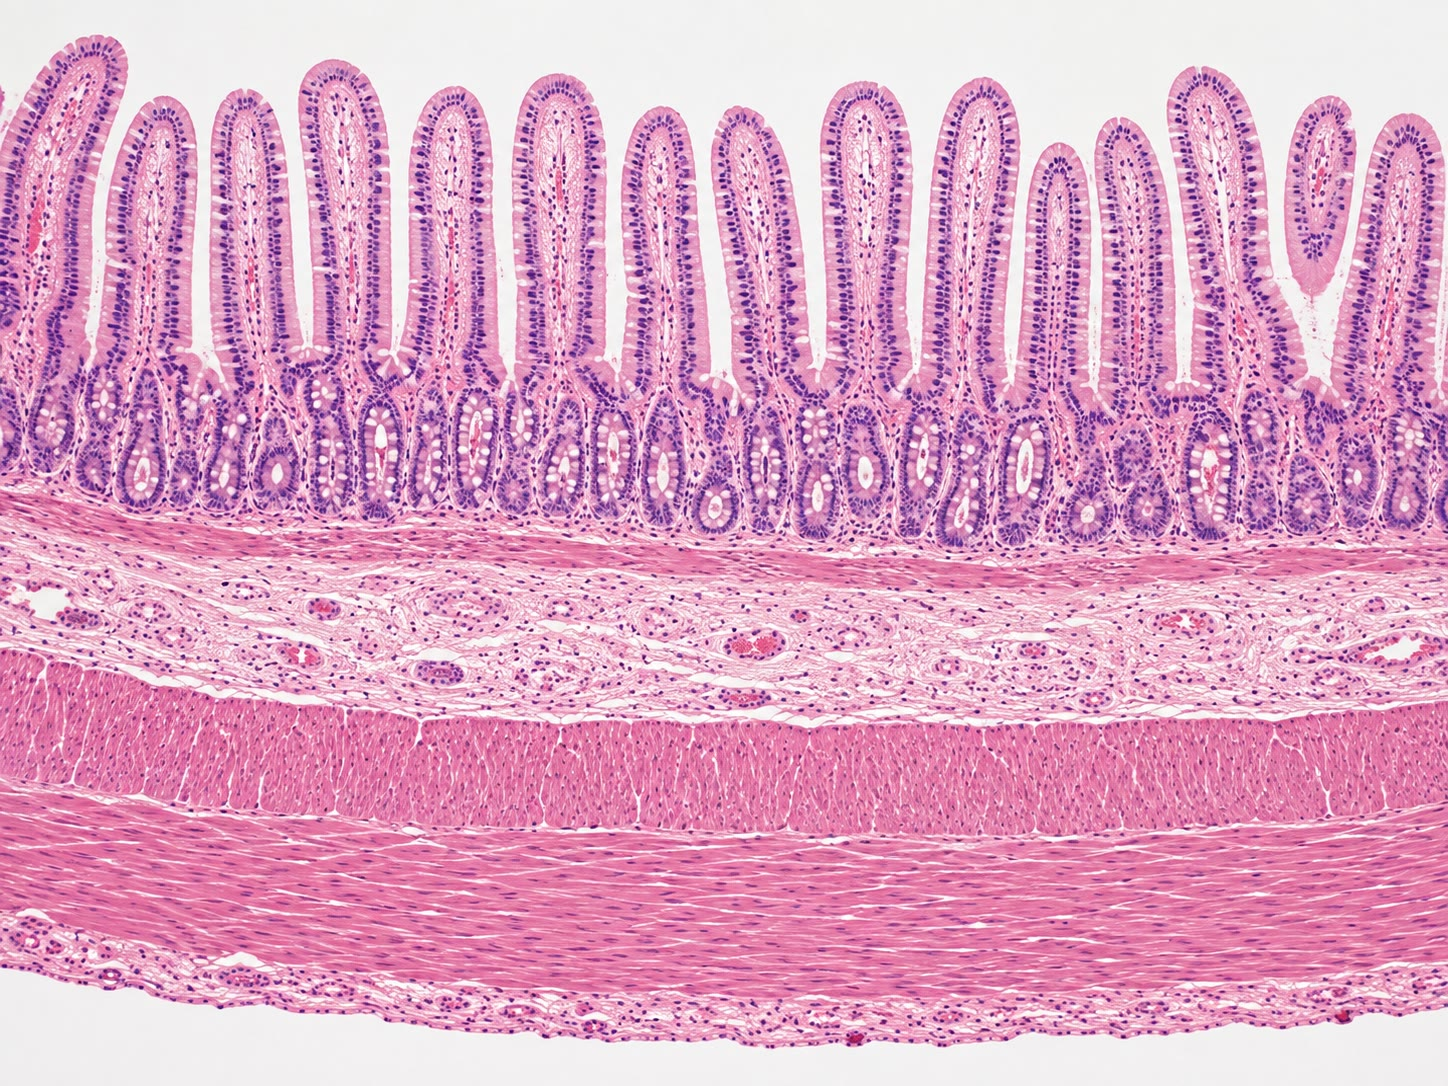
\includegraphics[width=0.53\linewidth]{images/book3/ai/fig-gut-wall-histology.jpg}};
  \begin{scope}[x={(img.south east)}, y={(img.north west)},
      every node/.style={font=\small}]
    \draw[omDef, thick] (0.50,0.985) -- (0.50,1.08) node[above] {lúmen};
    \draw[omDef, thick] (0.30,0.82) -- (-0.03,0.86) node[left, align=right] {vilosidade: epitélio\\ sobre tecido conjuntivo};
    \draw[omDef, thick] (0.40,0.58) -- (-0.03,0.56) node[left] {glândulas (criptas)};
    \draw[omDef, thick] (0.70,0.505) -- (1.03,0.56) node[right] {muscular da mucosa};
    \draw[omDef, thick] (0.70,0.42) -- (1.03,0.42) node[right] {submucosa};
    \draw[omDef, thick] (0.70,0.24) -- (1.03,0.26) node[right, align=left] {muscular: circular\\ e longitudinal};
    \draw[omDef, thick] (0.70,0.06) -- (1.03,0.06) node[right] {serosa};
  \end{scope}
\end{tikzpicture}

{\small Corte transversal da parede do intestino delgado. As
vilosidades da mucosa projetam-se para o lúmen; abaixo delas, as
glândulas, uma lâmina fina de músculo, a submucosa, as duas camadas da
muscular e a serosa. Quatro camadas, quatro tipos de \omterm{def:b1:body-plans-tissues:tissue}{tecido}, um \omterm{def:b1:mammal-organization:organ}{órgão}.}
\end{omfigure}

\begin{method}[Ler um corte histológico]\label{met:b1:body-plans-tissues:histology}
\begin{enumerate}
  \item Encontre a superfície livre ou o lúmen: o \omterm{def:b1:body-plans-tissues:epithelium}{epitélio} que o reveste
        é a primeira camada. Conte as fileiras de núcleos dele (simples
        ou estratificado) e observe a forma das células.
  \item Abaixo do \omterm{def:b1:body-plans-tissues:epithelium}{epitélio} procure a zona pálida e fibrosa, com núcleos
        esparsos e vasos: o \omterm{def:b1:body-plans-tissues:connective}{tecido conjuntivo}.
  \item O músculo aparece como feixes densos de células alongadas:
        estriado com núcleos periféricos (esquelético), estriado e
        ramificado (cardíaco), não estriado com um núcleo central
        (liso). Observe a direção das fibras em relação ao corte.
  \item O \omterm{def:b1:body-plans-tissues:nervous}{tecido nervoso}, na parede de um \omterm{def:b1:mammal-organization:organ}{órgão}, aparece como
        agrupamentos de corpos neuronais grandes e pálidos entre as
        camadas musculares.
  \item Nomeie o \omterm{def:b1:mammal-organization:organ}{órgão} pela sequência de camadas e pelas especializações
        da mucosa (vilosidades, glândulas, queratina).
\end{enumerate}
\end{method}

\begin{example}[A vilosidade como superfície de troca]\label{ex:b1:body-plans-tissues:villus}
Uma vilosidade do intestino delgado humano é um dedo de \qty{0.6}{mm} de
altura e \qty{0.15}{mm} de largura, coberto por uma única camada de
células prismáticas cujas faces apicais carregam, cada uma, cerca de
\qty{1500}{} microvilosidades. As vilosidades multiplicam a superfície
do tubo por cerca de sete e as microvilosidades por mais vinte: os
\qty{0.6}{m^2} de um tubo liso viram dezenas de metros quadrados de
\omterm{def:b1:body-plans-tissues:epithelium}{epitélio} absortivo com uma célula de espessura, cada célula a poucos
micrômetros de um capilar e de um vaso linfático no eixo conjuntivo da
vilosidade dela (\cref{ch:b1:digestion-absorption}). O \omterm{def:b1:body-plans-tissues:epithelium}{epitélio} é
renovado a partir das glândulas da base a cada quatro dias: a lâmina, as
junções e a polaridade dela são reconstruídas continuamente.
\end{example}

\begin{remark}[Os tecidos dos dois organismos-modelo]\label{rem:b1:body-plans-tissues:plants}
Os três sistemas de \omterm{def:b1:body-plans-tissues:tissue}{tecidos} da planta do
\cref{ch:b1:flowering-plant-organization} não têm equivalentes exatos
aqui. A epiderme dela é um \omterm{def:b1:body-plans-tissues:epithelium}{epitélio} pela função, mas as células dela são
seguradas por paredes, e não por junções; o \omterm{def:b1:flowering-plant-organization:tissues}{tecido fundamental} dela é ao
mesmo tempo de reserva, de sustentação e fotossintético; ela não tem
nem músculo nem nervo. Os quatro \omterm{def:b1:body-plans-tissues:tissue}{tecidos} do animal são a caixa de
ferramentas de um corpo que se move e percebe; os três da planta, de um
corpo que cresce.
\end{remark}

\section{Exercícios}

\begin{exercise}[$\star$]\label{exo:b1:body-plans-tissues:1}
Defina \omterm{def:b1:body-plans-tissues:symmetry}{simetria radial} e \omterm{def:b1:body-plans-tissues:symmetry}{simetria bilateral} e dê um animal de cada uma.
Qual delas acompanha a \omterm{def:b1:mammal-organization:bodyplan}{cefalização}, e por quê?
\end{exercise}

\begin{exercise}[$\star$]\label{exo:b1:body-plans-tissues:2}
Cite os três \omterm{def:b1:body-plans-tissues:layers}{folhetos embrionários} e um \omterm{def:b1:body-plans-tissues:tissue}{tecido} derivado de cada um.
\end{exercise}

\begin{exercise}[$\star$]\label{exo:b1:body-plans-tissues:3}
Liste os quatro tipos de \omterm{def:b1:body-plans-tissues:tissue}{tecido} com a característica definidora e uma
função de cada um.
\end{exercise}

\begin{exercise}[$\star$]\label{exo:b1:body-plans-tissues:4}
A partir da figura do \omterm{def:b1:body-plans-tissues:epithelium}{epitélio}, cite as quatro junções do ápice para a
base e a tarefa de cada uma.
\end{exercise}

\begin{exercise}[$\star\star$]\label{exo:b1:body-plans-tissues:5}
Um animal tem três \omterm{def:b1:body-plans-tissues:layers}{folhetos embrionários}, uma cavidade corporal
revestida de \omterm{def:b1:body-plans-tissues:layers}{mesoderma}, um tubo digestório completo, segmentos
semelhantes e nenhuma parte dura. Dê as características do plano dele
uma a uma e cite um grupo que se encaixe.
\end{exercise}

\begin{exercise}[$\star\star$]\label{exo:b1:body-plans-tissues:6}
Explique como uma minhoca se move usando o \omterm{def:b1:body-plans-tissues:layers}{celoma} como esqueleto, com as
duas camadas musculares de cada segmento.
\end{exercise}

\begin{exercise}[$\star\star$]\label{exo:b1:body-plans-tissues:7}
Compare o \omterm{def:b1:body-plans-tissues:segments}{exoesqueleto} do lagostim com o \omterm{def:b1:body-plans-tissues:segments}{endoesqueleto} da rã:
crescimento, proteção, inserção dos músculos e o limite de tamanho que
cada um impõe.
\end{exercise}

\begin{exercise}[$\star\star$]\label{exo:b1:body-plans-tissues:8}
Por que um \omterm{def:b1:body-plans-tissues:epithelium}{epitélio} precisa de junções oclusivas para ser uma \omterm{prop:b1:organism-environment:surfaces}{superfície
de troca} sob o controle do \omterm{def:b1:organism-environment:organism}{organismo}? O que aconteceria com a absorção
intestinal sem elas?
\end{exercise}

\begin{exercise}[$\star\star$]\label{exo:b1:body-plans-tissues:9}
Um corte mostra, do lúmen para fora: um \omterm{def:b1:body-plans-tissues:epithelium}{epitélio} prismático simples com
vilosidades, \omterm{def:b1:body-plans-tissues:connective}{tecido conjuntivo} frouxo, uma lâmina fina de músculo,
\omterm{def:b1:body-plans-tissues:connective}{tecido conjuntivo} denso, duas camadas musculares espessas e uma camada
externa fina. Nomeie o \omterm{def:b1:mammal-organization:organ}{órgão} e cada camada.
\end{exercise}

\begin{exercise}[$\star\star\star$]\label{exo:b1:body-plans-tissues:10}
A cartilagem não tem vasos sanguíneos e o osso tem muitos. Relacione
isso ao modo como cada um é nutrido, à rapidez com que cada um
cicatriza, e a onde cada um é usado no corpo.
\end{exercise}

\begin{exercise}[$\star\star\star$]\label{exo:b1:body-plans-tissues:11}
Um fármaco bloqueia a formação das junções oclusivas no \omterm{def:b1:body-plans-tissues:epithelium}{epitélio}
intestinal. Preveja os efeitos dele sobre a absorção, sobre a composição
do \omterm{def:b1:organism-environment:milieu}{meio interno} e sobre a infecção, usando as propriedades dos
\omterm{def:b1:body-plans-tissues:epithelium}{epitélios}.
\end{exercise}

\begin{exercise}[$\star\star\star$]\label{exo:b1:body-plans-tissues:12}
``Um \omterm{def:b1:mammal-organization:bodyplan}{plano de organização} é um conjunto de restrições, e não um
projeto.'' Discuta em um parágrafo, usando a muda dos artrópodes, o
tamanho dos insetos, os segmentos dos vertebrados e o sentido da tabela
deste capítulo.
\end{exercise}

\section{Problema: A parede do intestino delgado}

\begin{problem}[{Problema de fim de semana --- uma série histológica do
intestino delgado humano lida do tubo até a microvilosidade: camadas,
vilosidades, células, junções e renovação, terminando na superfície
absortiva de uma única vilosidade}]
\label{pb:b1:body-plans-tissues:1}
O intestino delgado humano é um tubo de \qty{6}{m} de comprimento e
\qty{3}{cm} de diâmetro interno. As pregas circulares da parede dele
triplicam a superfície do tubo liso. A mucosa dele carrega \qty{25}{}
vilosidades por milímetro quadrado de superfície pregueada, cada uma um
cilindro de \qty{0.6}{mm} de altura e \qty{0.15}{mm} de diâmetro. As
vilosidades são cobertas por células prismáticas cuja face apical é um
quadrado de \qty{5}{\micro m} de lado; cada face apical carrega
\qty{1500}{} microvilosidades, cilindros de \qty{1}{\micro m} de
comprimento e \qty{0.1}{\micro m} de diâmetro. O \omterm{def:b1:body-plans-tissues:epithelium}{epitélio} é renovado a
cada \qty{4}{} dias.

\medskip
\noindent\textbf{Parte I --- As camadas.}
Um corte transversal é examinado ao microscópio.
\begin{enumerate}
  \item Liste as quatro camadas da parede, do lúmen para fora, e os
        tipos de \omterm{def:b1:body-plans-tissues:tissue}{tecido} de cada uma.
  \item O corte mostra vilosidades. De que região do tubo digestório ele
        é? O que um corte do estômago mostraria no lugar?
  \item Entre as duas camadas musculares da muscular há agrupamentos de
        células grandes e pálidas. O que elas são e o que controlam?
  \item Explique por que as duas camadas musculares correm em direções
        perpendiculares.
\end{enumerate}

\medskip
\noindent\textbf{Parte II --- Superfícies.}
\begin{enumerate}[resume]
  \item Calcule a superfície interna do tubo liso.
  \item Calcule a superfície depois das pregas circulares.
  \item Calcule a superfície lateral de uma vilosidade (cilindro,
        ignorando a ponta).
  \item Calcule a superfície de vilosidades por milímetro quadrado de
        mucosa pregueada e o fator pelo qual as vilosidades multiplicam
        a superfície.
  \item Calcule a superfície depois das vilosidades.
  \item Calcule a superfície lateral de uma microvilosidade e a das
        \qty{1500}{} de uma célula.
  \item Calcule o fator pelo qual as microvilosidades multiplicam a
        superfície apical de uma célula.
  \item Calcule a superfície absortiva total do intestino delgado.
\end{enumerate}

\medskip
\noindent\textbf{Parte III --- Células.}
\begin{enumerate}[resume]
  \item Calcule o número de células epiteliais que cobrem uma
        vilosidade.
  \item Calcule o número de vilosidades do intestino delgado e o número
        de células epiteliais que as cobrem.
  \item O \omterm{def:b1:body-plans-tissues:epithelium}{epitélio} é renovado a cada \qty{4}{} dias. Quantas células são
        descamadas para o lúmen por dia, e por segundo?
  \item Onde as células de reposição são produzidas, e o que isso diz
        sobre a posição das células que se dividem em relação às que
        absorvem?
  \item Uma célula epitelial tem \qty{25}{\micro m} de altura. Calcule o
        volume de \omterm{def:b1:body-plans-tissues:epithelium}{epitélio} do intestino delgado e a massa dele
        (densidade \qty{1.05}{g/cm^3}).
\end{enumerate}

\medskip
\noindent\textbf{Parte IV --- Junções, matriz e a vilosidade.}
\begin{enumerate}[resume]
  \item Cada célula é vedada às vizinhas por uma junção oclusiva que
        corre em volta do ápice dela. Calcule o comprimento de junção
        oclusiva por célula e o comprimento total no intestino delgado.
  \item Explique por que uma substância do lúmen só pode chegar ao
        sangue atravessando duas membranas celulares.
  \item O eixo da vilosidade é \omterm{def:b1:body-plans-tissues:connective}{tecido conjuntivo} frouxo com uma rede
        capilar e um vaso linfático central. Cite os dois tipos de fibra
        extracelular que ele contém e a célula que as secreta.
  \item Cite o \omterm{def:b1:body-plans-tissues:layers}{folheto embrionário} de origem do \omterm{def:b1:body-plans-tissues:epithelium}{epitélio} e o do eixo.
  \item A vilosidade também contém um feixe de músculo liso que a faz
        encurtar ritmicamente. Proponha a função dele.
  \item Uma doença achata as vilosidades (a superfície volta à do tubo
        pregueado). Por qual fator a superfície absortiva cai, e quais
        são as consequências?
  \item Calcule a superfície absortiva de uma vilosidade com as
        microvilosidades dela, em milímetros quadrados.
  \item Enuncie o resultado: a superfície absortiva de uma única
        vilosidade e o número de vilosidades do intestino delgado.
\end{enumerate}
\end{problem}
